
\section{Overview}\label{sect:Overview}

This tutorial is intended to provide a introduction to the basics of Markov chain Monte Caro (MCMC) using the  Metropolis-Hastings algorithm. This will provide a brief introduction to MCMC moves as well as prior distributions. We begin with a simple example of estimating the probability distribution of an archer's ability to shoot at a target, and the distance those arrows land from the center. We will simulate data using this example and attempt to estimate the posterior distribution using a variety of MCMC moves. 

\bigskip
\subsection{Learning Outcomes}
\begin{itemize}
\item Understand and implement the Metropolis-Hastings MCMC algorithm
\item Understand the difference and utility of various MCMC moves 
\item Begin to develop an intuition regarding the use of different priors 
\end{itemize}

\subsection{Required Software}\label{subsect:Overview-Requirements}

This tutorial requires that you download and install the latest release of \RevBayes \citep{Hoehna2017a}, which is available for Mac OS X, Windows, and Linux operating systems. 
Directions for downloading and installing the software are available on the program webpage:
%\begin{center}
\href{http://revbayes.com/}{http://revbayes.com}.
%\end{center} 

The exercise provided also requires additional programs for editing text files and visualizing output. 
The following are very useful tools for working with \RevBayes:
\begin{itemize}[noitemsep,topsep=0pt]
\item A good text editor -- if you do not already have one that you like, we recommend one that has features for syntax coloring, easy navigation between different files, line numbers, etc.
Good options include \href{http://www.sublimetext.com/}{\tt Sublime Text} or \href{https://atom.io/}{Atom}, which are available for Mac OSX, Windows, and Linux.
\item \href{http://tree.bio.ed.ac.uk/software/tracer/}{\tt Tracer} -- for visualizing and assessing numerical parameter samples from \RevBayes
\end{itemize}

\bigskip
\section{Introduction}\label{sect:Introduction}




\newpage
\section{Modeling an archer's shots on a target}\label{sect:Exercise}

Introduction to problem. Include within here the distribution the shots are fired under and the first prior distribution. Might be worth showing some similar figures to the ones in Paul's Woods Hole powerpoint here to illustrate points. Also would be a a place to explain the idea of a conjugate prior and why they are useful. 

\medskip
\subsection{Tutorial Format}\label{subsect:Exercise-Format}

This tutorial follows a specific format for issuing instructions and information.

{\begin{framed}
The boxed instructions guide you to complete tasks that are not part of the \RevBayes syntax, but rather direct you to create directories or files or similar.
\end{framed}}

Information describing the commands and instructions will be written in paragraph-form before or after they are issued.

All command-line text, including all \Rev syntax, are given in \cl{monotype font}. 
Furthermore, blocks of \Rev code that are needed to build the model, specify the analysis, or execute the run are given in separate shaded boxes.
For example, we will instruct you to create a constant node called \cl{rho} that is equal to \cl{1.0} using the \cl{<-} operator like this:
{\tt \begin{snugshade*}
\begin{lstlisting}
rho <- 1.0
\end{lstlisting}
\end{snugshade*}}

It is important to be aware that some PDF viewers may render some characters given as \colorbox{shadecolor}{\tt{Rev commands}} differently. 
Thus, if you copy and paste text from this PDF, you may introduce some incorrect characters. 
Because of this, we recommend that you type the instructions in this tutorial or copy them from the scripts provided. 


\medskip
\subsection{Data and Files}\label{subsect:Exercise-DataFiles}

{\begin{framed}
On your own computer or your remote machine, create a directory called {\textcolor{red}{\cl{RB\_MyFirstMCMC\_Tutorial}}} (or any name you like).

\end{framed}}

In this tutorial we will be simulating our own data using \RevBayes. Explain how to simulate data in Rev. We will be simulating data. Let's assume from the above archery example that our archer's true ability has their arrows landing with a mean of 0 and a variance of 1. Let's say they shoot six arrows. We do this in \RevBayes like this:

 {\tt \begin{snugshade*}
\begin{lstlisting}
num_arrows <- 6
mu <- 0.0
var <- 1
\end{lstlisting}
\end{snugshade*}}



\bigskip
\subsection{Getting Started with MCMC\label{subsect:Exercise-GetStart}}

Explain what MCMC does here.

\subsubsection{Metropolis-Hastings algorithm}

Go through outline of algorithm steps. explain proposal distributions. Then go into a step-by-step on how to write a MH-algorithm in Rev. First write the functions for the likelihood and the prior. 

Likelihood function:

 {\tt \begin{snugshade*}
\begin{lstlisting}
function RealPos likelihood(v){
	nu = 0
	for(i in 1:num_arrows){
		nu += (arrows[i] - mu)^2
	}
	l = 1 / dgamma(v, (num_arrows + 2*alpha) / 2, (num_arrows + 2*beta) / 2)
	return l
}

\end{lstlisting}
\end{snugshade*}}

Prior function: 

{\tt \begin{snugshade*}
 \begin{lstlisting}
function RealPos priorVar(v_prime){
	pv_inv = dgamma(v, alpha, beta, log=false)
	pv = 1 / pv_inv # we would like inv gamma distribution
	return pv
}
\end{lstlisting}
\end{snugshade*}}



Set the number of iterations, draw intitial values for prior. And then write the for loop defining the algorithm itself. 
Draw an initial value for our prior:

{\tt \begin{snugshade*}
 \begin{lstlisting}
alpha <- 1
beta <- 1

v <- 1 / rgamma(1, a, b)[1]
\end{lstlisting}
\end{snugshade*}}

Set number of iterations of our MCMC and setup writing our ouput:

{\tt \begin{snugshade*}
 \begin{lstlisting}
niter = 10000
write("iteration","p","\n",file="archery_MH.log")
write(0,v,"\n",file="archery_MH.log",append=TRUE)
\end{lstlisting}
\end{snugshade*}}


Metropolis Hastings Algorithm:

{\tt \begin{snugshade*}
 \begin{lstlisting}
for(i in 1:niter){
	v_prime <- rexp(n=1, 1.0)[1]
    
	R <- (likelihood(v_prime) / likelihood(v)) * ( priorVar(v_prime) / priorVar(v))
	u <- runif(1,0,1)[1]
	if(u < R){
		v <- v_prime
	}

	write(rep,v,"\n",file="archery_MH.log",append=TRUE)
}
\end{lstlisting}
\end{snugshade*}}



%TODO Stuff about how to start or Rev basics?

%We will complete this analysis in \RevBayes by entering the \Rev code interactively. 
%
%Note that some PDF viewers render some characters differently and if you copy/paste directly from this document, you may introduce erroneous characters. 
%This can cause commands to fail. 
%For learning, it's often better to `live code' and type the commands in manually, rather than copying and pasting. 
%
%Hints for navigating in the \RevBayes console:
%\begin{itemize}[noitemsep,topsep=0pt]
%    \item \cl{Ctrl+A} -- jump to the beginning of the line
%    \item \cl{Ctrl+E} -- jump to the end of the line
%    \item Pressing the up key will pull up previous commands, and allow you to edit them
%    \item If you enter the first few letters of a \RevBayes keyword and then the \textsc{Tab} key, this will `autocomplete' the remaining letters.
%    \item Help -- if you type \cl{?} followed immediately by a \RevBayes keyword, this will print the help pages for that keyword to the screen. (Example \cl{?dnBDP})
%\end{itemize}
%%In \RevBayes, \cl{Ctrl+A} allows you to jump to the start of the command, if you need to delete extra characters from the front of a line. \cl{Ctrl+E} allows you to jump to the end of a command. Pressing the up key will pull up previous commands, and allow you to edit them. If you do choose to copy and paste in commands, doing that from the tutorial script file will cause fewer errors. 

\bigskip

\section{Exercises}

\subsection{Using different priors}

Suppose we know little about the variance of some archer. In that case, we have little prior belief and a very flat prior might be a good choice. Our conjugate prior is convenient here as the Inverse-Gamma distribution is relatively flat when $\alpha = \beta$ are very small. Estimate the posterior density with alpha and beta as very small values (perhaps try 0.001). compare with your previous posterior distribution.

Another flat distribution may be more obvious (the uniform) try this one as well. What are some limitations to the Uniform? 

\subsection{Defining different MCMC moves}

Previously, we had been using random draws from (whatever) distribution for the prior. There are lots of possibilities for doing this. We can test how efficient these moves are at sampling our target distributions. Some are far more efficient than others. Code up all of the moves in RevBayes.

\subsubsection{Random draw}
introduce weights here. (maybe have an aside explaining using a 2 parameter model?)
\subsubsection{Sliding move}
Explain about $\delta$ (the tuning parameter). What values are good/bad for this? Explain about how to tune and the purpose of it.

\subsubsection{Scaling move}
Similarly, explain the tuning parameter for this move. Also, this move is asymmetric so explain more about the calculation of the Hastings ratio. 

Compare the three different moves in tracer.
%\subsection{Creating \Rev Files}\label{subsect:Exercise-CreatingFiles}
%
%{\begin{framed}
%Create a new directory (in \cl{RB\_TotalEvidenceDating\_FBD\_Tutorial}) called {\textcolor{red}{\cl{scripts}}}. (If you do not have this folder, please refer to the directions in section \ref{subsect:Exercise-DataFiles}.)
%\end{framed}}
%
%When you execute \RevBayes in this exercise, you will do so within the main directory you created, \cl{RB\_TotalEvidenceDating\_FBD\_Tutorial}, thus, if you are using a Unix-based operating system, we recommend that you add the \RevBayes binary to your path.
%
%
%For complex models and analyses, it is best to create \Rev script files that will contain all of the model parameters, moves, and functions. 
%In this exercise, you will work primarily in your text editor\footnote{In section \ref{subsub:Req-Software} we offer a recommendation for a text editor.} and create a set of modular files that will be easily managed and interchanged.
%You will write the following files from scratch and save them in the \cl{scripts} directory/
%All of the files that you will create are also provided in the \RevBayes tutorial repository\footnote{\url{https://github.com/revbayes/revbayes_tutorial/tree/master/RB_MyFirstMCMC_Tutorial/scripts}}. 
%Please refer to these files to verify or troubleshoot your own scripts. 

%{\footnotesize{This file is provided in the \RevBayes tutorial repository: \href{https://github.com/revbayes/revbayes_tutorial/blob/master/RB_TotalEvidenceDating_FBD_Tutorial/scripts/mcmc_TEFBD.Rev}{\cl{mcmc\_TEFBD.Rev}}.}}

%{\begin{framed}
%Navigate to \url{http://tgvaughan.github.io/icytree} and open the file \cl{output/bears.mcc.tre} in {\tt IcyTree}.
%
%\QUEST Try to replicate the tree in Fig.\ \ref{fig:IcyTreeSumm}. (Hint: \mi{Style\textrightarrow Mark Singletons})
%Why might a node with a sampled ancestor be referred to as a singleton? 
%
%\QUEST How can you see the names of the fossils that are putative sampled ancestors?
%
%\QUEST Try mousing over different branches (see Fig.\ \ref{fig:IcyTreeScreenshort}).
%What are the fields telling you?
%%Is the age of the \textit{Kretzoiarctos beatrix} fossil the same as what was shown in {\tt Tracer}? 
%
%\QUEST What is the posterior probability that \textit{Zaragocyon daamsi} is a sampled ancestor?
%
%Another newly available web-based tree viewer is \href{http://phylogeny.io/}{Phylogeny.IO} \citep{Jovanovic2016}. 
%Try this site for a different way to view the tree.
%\end{framed}}



%TODO more here, create final tree image


%\begin{figure}[h!]
%\fbox{%
%\begin{minipage}{\textwidth}\centering
%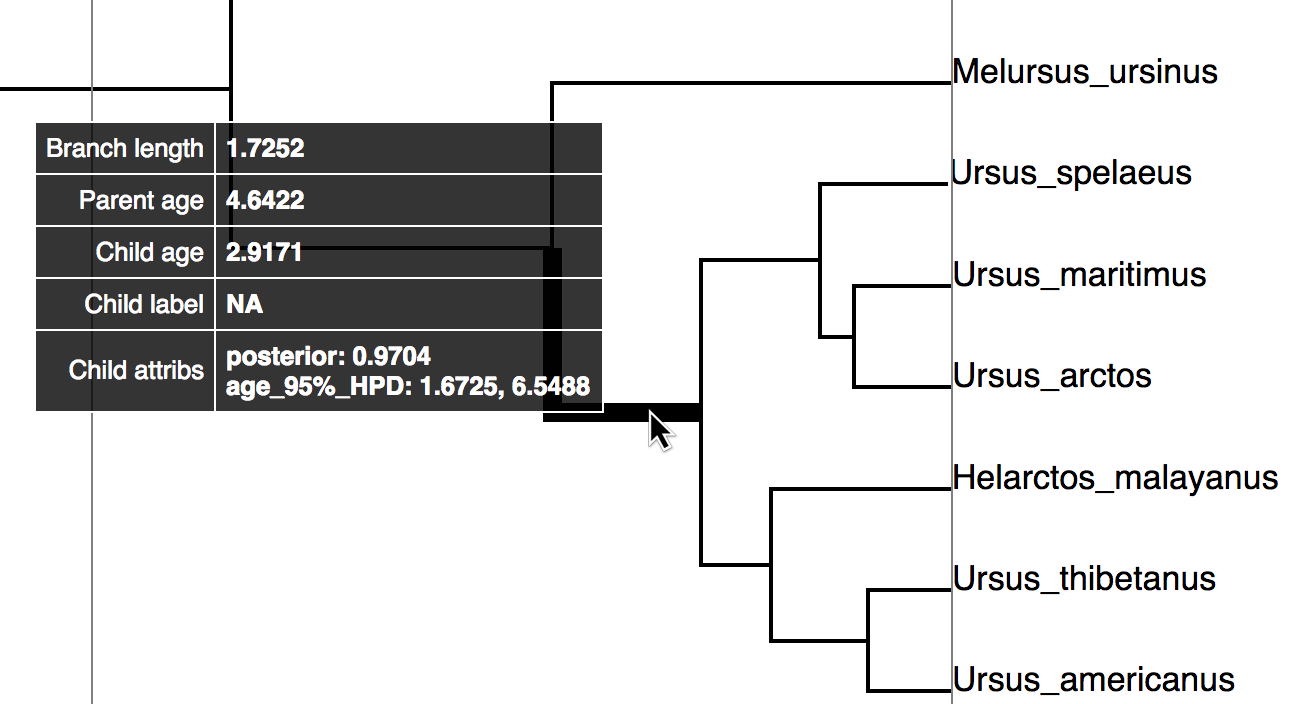
\includegraphics[scale=0.45, angle=0]{\ResourcePath figures/branch_highlight.png}
%\caption{\small Screenshot of highlighting a branch in {\tt IcyTree} showing child node attributes, including the clade posterior probability and the 95\% highest posterior density (HPD) age interval.}
%\end{minipage}}
%\label{fig:IcyTreeScreenshort}
%\end{figure}



%TODO IcyTree

\bibliographystyle{sysbio}
\bibliography{\GlobalResourcePath refs}
